\chapter{Suggestions to Improve The Existing System} \label{suggestions}

\section{System Perspective}

\begin{figure}[H]
    \centering
    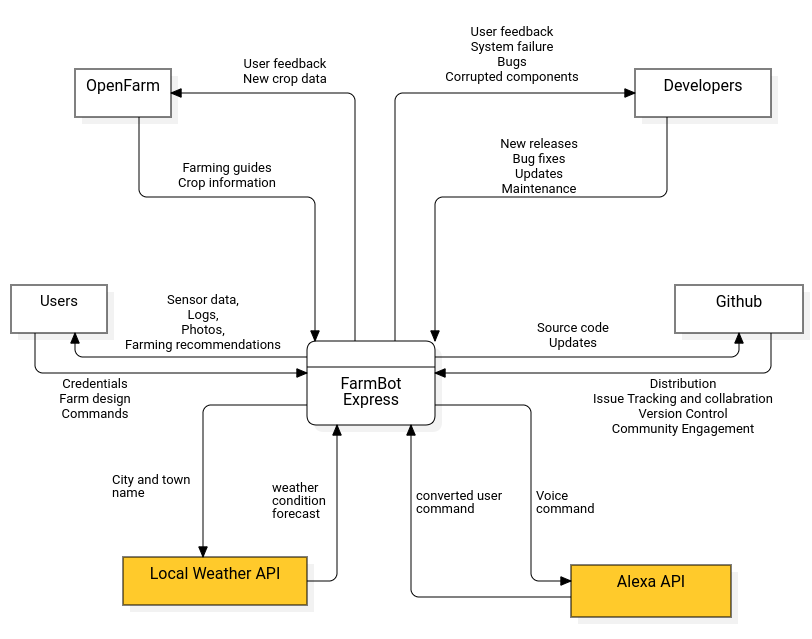
\includegraphics[width=1\textwidth]{UML Diagrams/SuggestedContextDiagram.png}
    \caption{Improved Context Diagram}
    \label{fig:suggested_context}
\end{figure}
The improved context diagram is shown in Figure \ref{fig:suggested_context}.
It now has Local Weather API and Alexa API as new external entities. The system can get weather data from \textbf{Local Weather API} and add this data to its smart decision-making process. Also, the system can communicate with \textbf{Alexa API} to provide voice command support. 

\section{External Interfaces}

\begin{figure}[H]
    \centering
    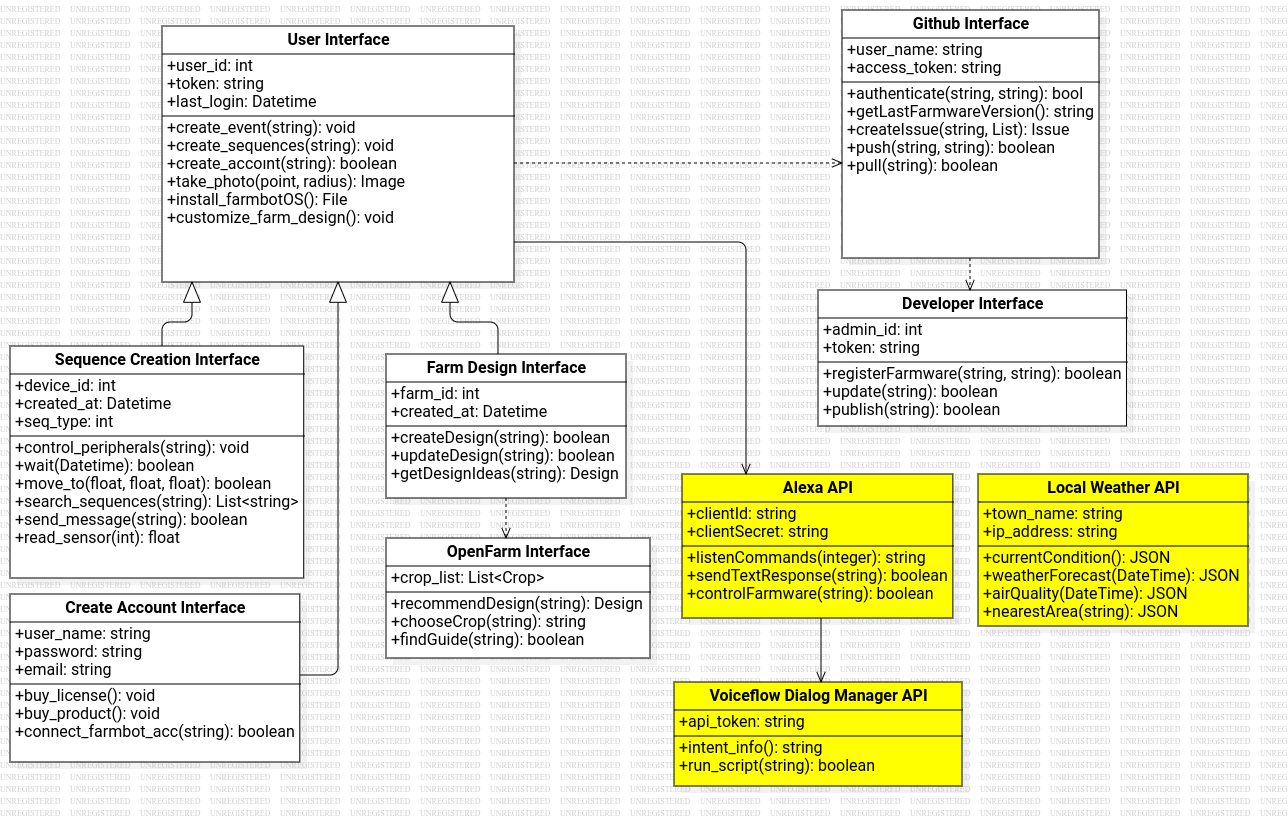
\includegraphics[width=1\textwidth]{UML Diagrams/SuggestedClassDiagram.png}
    \caption{Improved External Interface Diagram}
    \label{fig:suggested_external}
\end{figure}

\begin{itemize}
    \item \textbf{Local Weather API:} The system can get the current weather, temperature, humidity, and wind speed data from this API. The data can be used to make better decisions for the farm.
    \item \textbf{Alexa API:} The system can communicate with this Alexa API (provided by Amazon) to provide voice command support. The user can give voice commands to the system, and the system can respond to these commands. The vocal input goes into the Alexa API and redirects to the Voiceflow API. The Voiceflow API processes the vocal input and sends the processed data to the system.
    \item \textbf{Voiceflow Dialog Manager API}: This newly introduced API gets its input from Alexa API and runs JavaScript code triggering the commands.
\end{itemize}



\section{Functions}

\begin{figure}[H]
    \centering
    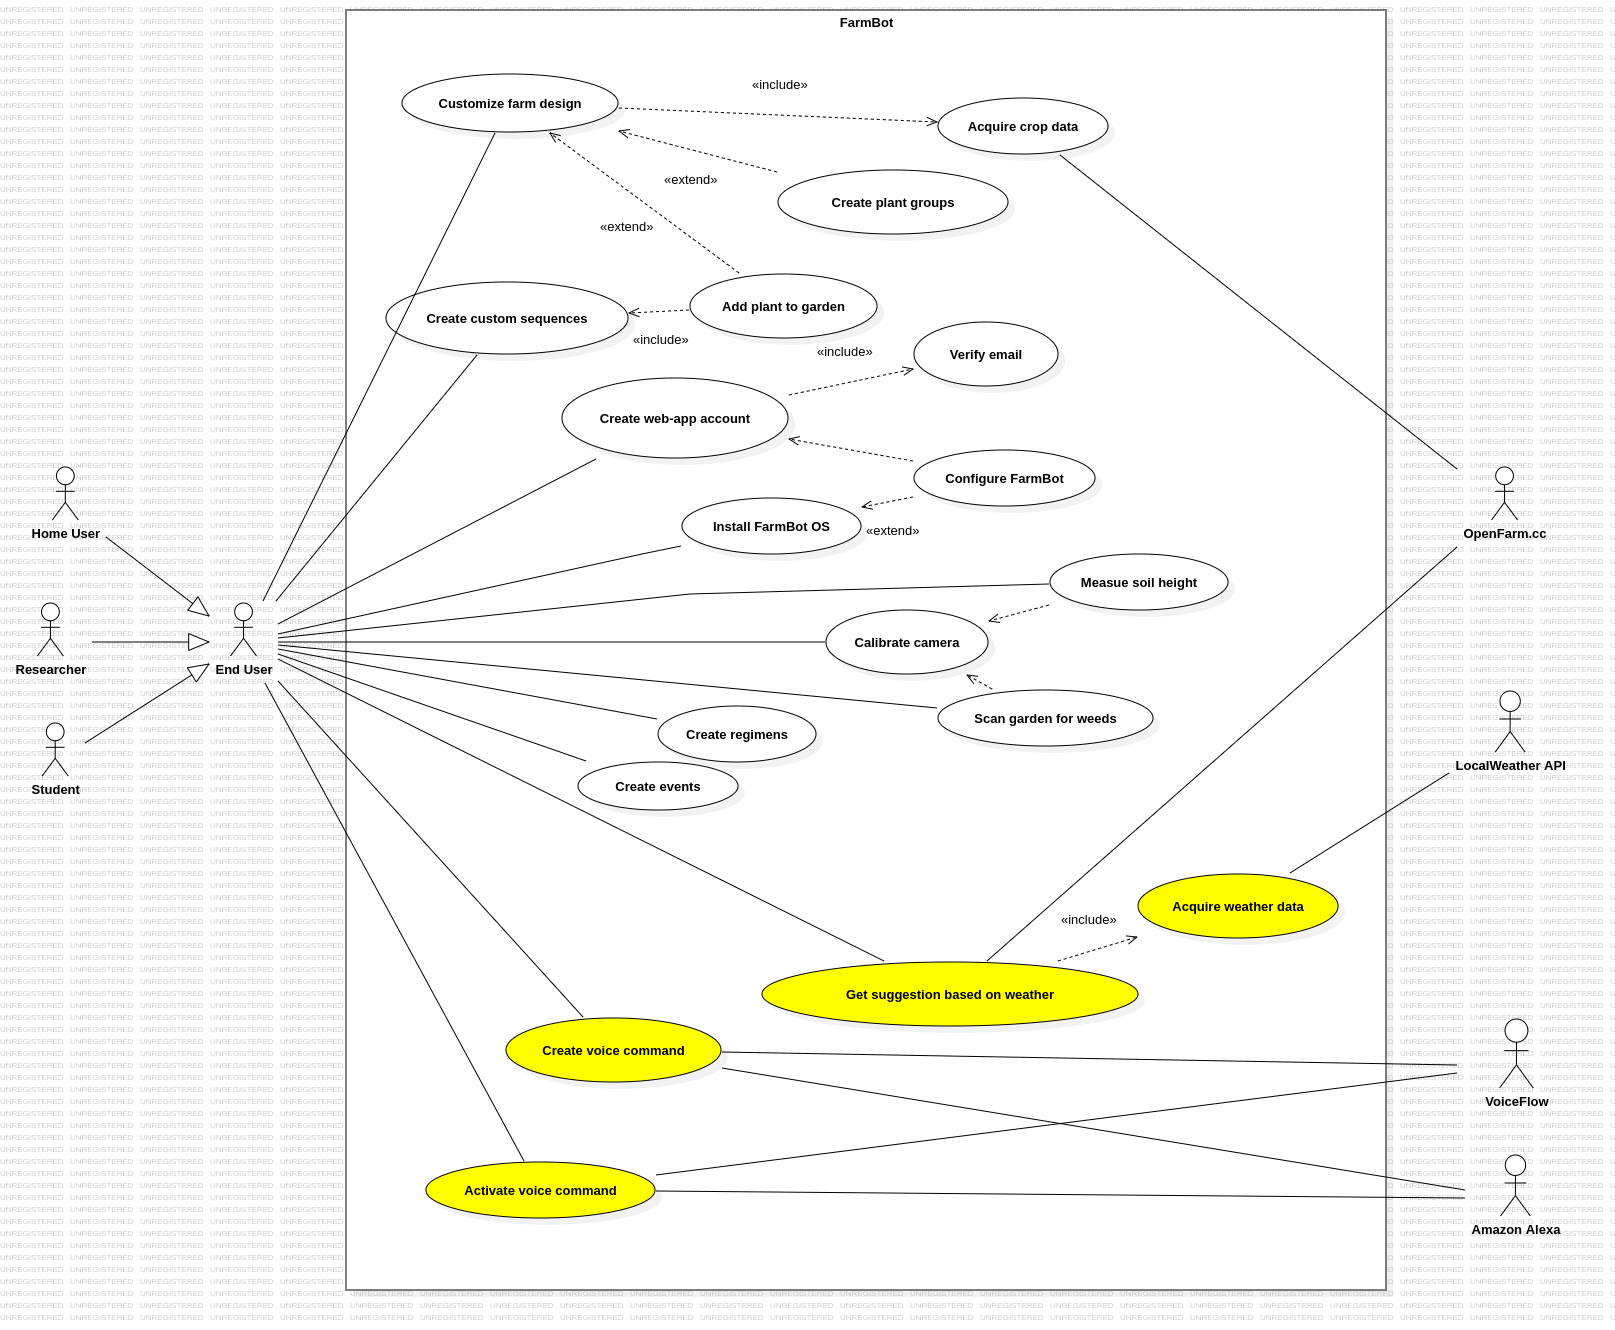
\includegraphics[width=1\textwidth]{UML Diagrams/UseCaseDiagram_suggestions.png}
    \caption{Improved Use Case Diagram}
    \label{fig:usecasediagram-suggestions}
\end{figure}

% Please add the following required packages to your document preamble:
% \usepackage{graphicx}
\begin{table}[H]
\centering
\resizebox{\textwidth}{!}{%
\begin{tabular}{|l|l|}
\hline
\textbf{Use case name}    & Activate voice command                                                           \\ \hline
\textbf{Actors}           & End User, VoiceFlow, Amazon Alexa                                                \\ \hline
\textbf{Description} &
  \begin{tabular}[c]{@{}l@{}}End user talks with the virtual assistant Alexa integrated with VoiceFlow to\\ run farming sequences\end{tabular} \\ \hline
\textbf{Preconditions} &
  \begin{tabular}[c]{@{}l@{}}User has a Amazon Alexa device\\ User is logged on the device\\ User is able to talk\\ User has created sequences on FarmBot web-app\end{tabular} \\ \hline
\textbf{Data}             & User voice, user FarmBot sequences                                               \\ \hline
\textbf{Response}         & FarmBot starts executing sequence                                                \\ \hline
\textbf{Stimulus}         & User says the word "Alexa" to wake device up                                     \\ \hline
\textbf{Normal Flow} &
  \begin{tabular}[c]{@{}l@{}}1. User tells the sequence they want to execute e.g. "FarmBot, run watering sequence."\\ 2. Alexa processes the command and sends it to VoiceFlow\\ 3. VoiceFlow sends request to execute sequence to FarmBot web-app\\ 4. FarmBot starts executing sequence\end{tabular} \\ \hline
\textbf{Alternative Flow} & -                                                                                \\ \hline
\textbf{Exception Flow}   & 3. If sequence does not exist, Alexa notifies the user and FarmBot does nothing. \\ \hline
\textbf{Post Conditions}  & Sequence must have started executing                                             \\ \hline
\textbf{Comments}         & -                                                                                \\ \hline
\end{tabular}%
}
\caption{Tabular description of Activate voice command use case}
\label{tab:activate-voice-command}
\end{table}

\begin{figure}[H]
    \centering
    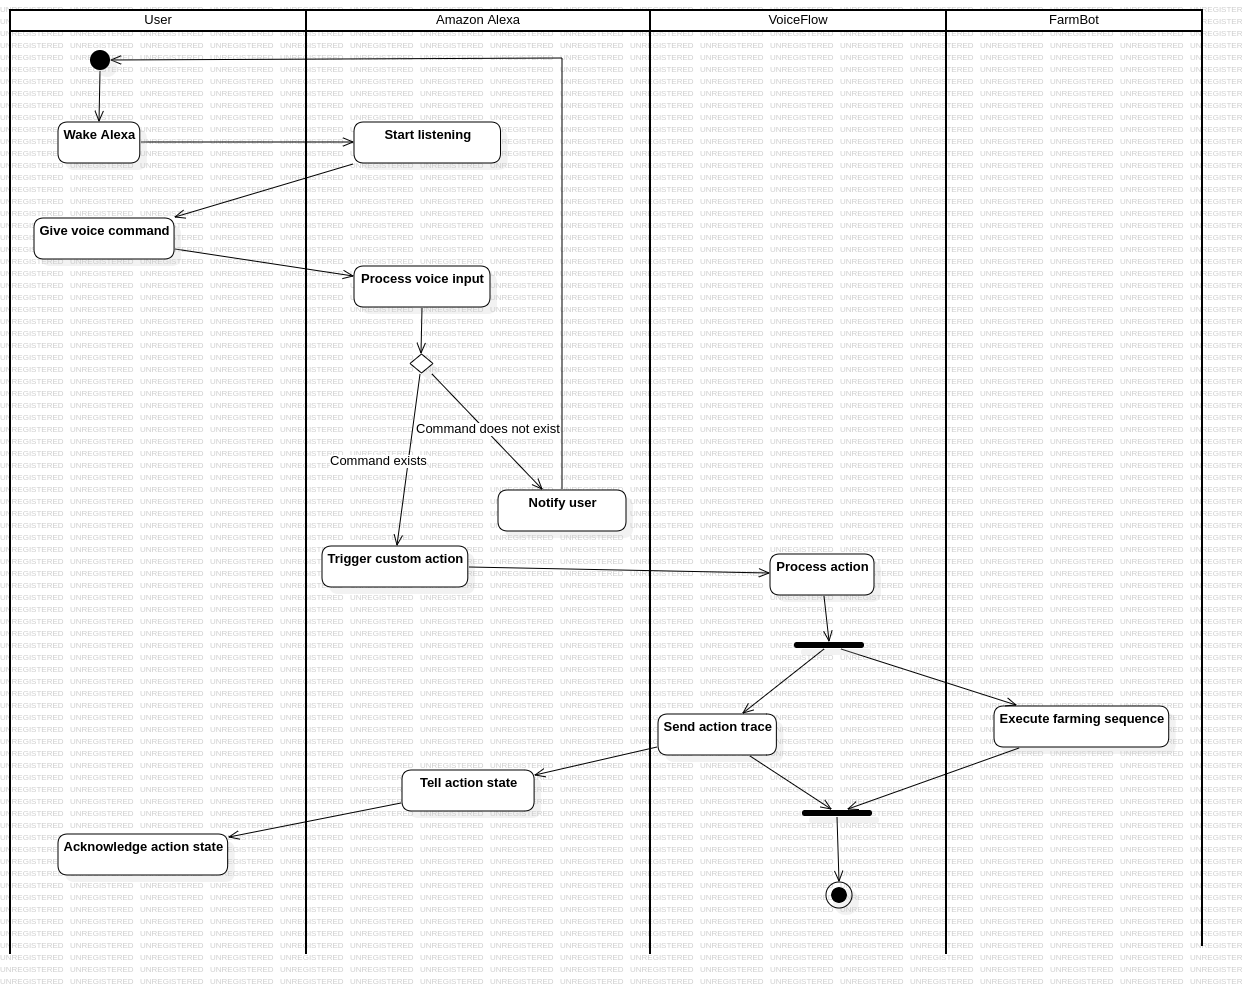
\includegraphics[width=1\textwidth]{UML Diagrams/ActivityDiagram_activatevoicecommand.png}
    \caption{Activity Diagram for "Activate voice command" use case}
    \label{fig:activity-diagram-activate-voice-command}
\end{figure}

% Please add the following required packages to your document preamble:
% \usepackage{graphicx}
\begin{table}[H]
\centering
\resizebox{\textwidth}{!}{%
\begin{tabular}{|l|l|}
\hline
\textbf{Use case name}    & Create voice command                                                                       \\ \hline
\textbf{Actors}           & End User, VoiceFlow, Amazon Alexa                                                          \\ \hline
\textbf{Description}      & User creates commands that execute farming sequences using Alexa integrated with VoiceFlow \\ \hline
\textbf{Preconditions} &
  \begin{tabular}[c]{@{}l@{}}User has an account on VoiceFlow\\ User has an account on Alexa Developer platform\end{tabular} \\ \hline
\textbf{Data}             & NLU information (intents, entities)                                                        \\ \hline
\textbf{Response}         & Amazon Alexa responds and executes the correct sequence                                    \\ \hline
\textbf{Stimulus}         & -                                                                                          \\ \hline
\textbf{Normal Flow} &
  \begin{tabular}[c]{@{}l@{}}1. User creates a VoiceFlow project\\ 2. User creates intents within the project eg. "water\_intent"\\ 3. User creates an Alexa Skill on Alexa Developer platform\\ 4. User replicates the VoiceFlow NLU (Natural Language Understanding) in the Alexa skill\end{tabular} \\ \hline
\textbf{Alternative Flow} & -                                                                                          \\ \hline
\textbf{Exception Flow}   & -                                                                                          \\ \hline
\textbf{Post Conditions}  & Alexa and VoiceFlow must be integrated and commands must be executing                      \\ \hline
\textbf{Comments} &
  \begin{tabular}[c]{@{}l@{}}By integrating Alexa with VoiceFlow users can activate voice commands in order to execute\\ certain farming sequences\end{tabular} \\ \hline
\end{tabular}%
}
\caption{Tabular description of Create voice command use case}
\label{tab:create-voice-command}
\end{table}

% Please add the following required packages to your document preamble:
% \usepackage{graphicx}
\begin{table}[H]
\centering
\resizebox{\textwidth}{!}{%
\begin{tabular}{|l|l|}
\hline
\textbf{Use case name}    & Acquire weather data                                                              \\ \hline
\textbf{Actors}           & Local Weather API                                                                 \\ \hline
\textbf{Description} &
  \begin{tabular}[c]{@{}l@{}}Weather data is acquired from Local Weather API including current weather, temperature,\\ humidity, and wind speed data to use for farming action suggestions\end{tabular} \\ \hline
\textbf{Preconditions} &
  \begin{tabular}[c]{@{}l@{}}FarmBot has city and town name configuration set\\ FarmBot is authenticated to Weather API\end{tabular} \\ \hline
\textbf{Data}             & Current weather, temparature, humidity, wind speed                                \\ \hline
\textbf{Response}         & Weather information is returned                                                   \\ \hline
\textbf{Stimulus}         & -                                                                                 \\ \hline
\textbf{Normal Flow} &
  \begin{tabular}[c]{@{}l@{}}1. Web-app provides location data (city, town name)\\ 2. Web-app provides number of days of forecast\\ 3. Web-app makes a request to the Local Weather API\\ 4. Weather information is returned\end{tabular} \\ \hline
\textbf{Alternative Flow} & 2. If number of days is not provided, the request is defaulted to monthly average \\ \hline
\textbf{Exception Flow}   & 1. If location data is not provided, request is rejected.                         \\ \hline
\textbf{Post Conditions}  & Weather information must be available to the web-app                              \\ \hline
\textbf{Comments}         & -                                                                                 \\ \hline
\end{tabular}%
}
\caption{Tabular description of Acquire weather data use case}
\label{tab:acquire-weather-data}
\end{table}

\begin{figure}[H]
    \centering
    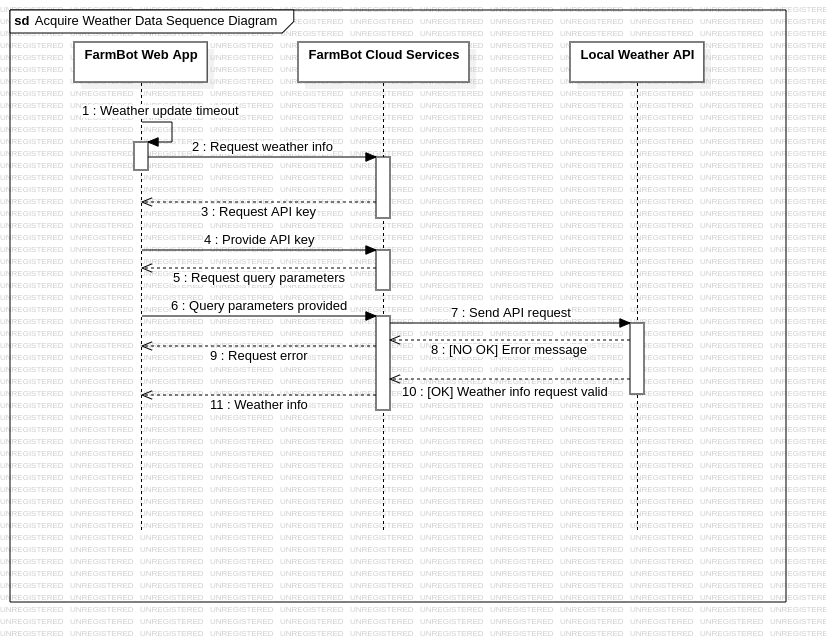
\includegraphics[width=1\textwidth]{UML Diagrams/SequenceDiagram_acquireweatherdata.png}
    \caption{Sequence Diagram for "Acquire weather data" use case}
    \label{fig:acquire-weather-data}
\end{figure}

% Please add the following required packages to your document preamble:
% \usepackage{graphicx}
\begin{table}[H]
\centering
\resizebox{\textwidth}{!}{%
\begin{tabular}{|l|l|}
\hline
\textbf{Use case name} &
  Get suggestion based on weather \\ \hline
\textbf{Actors} &
  OpenFarm.cc, End User, Local Weather API \\ \hline
\textbf{Description} &
  \begin{tabular}[c]{@{}l@{}}Farming action suggestions are provided to the user based on the acquired weather data,\\ and available crop information\end{tabular} \\ \hline
\textbf{Preconditions} &
  \begin{tabular}[c]{@{}l@{}}Weather API is not down\\ OpenFarm is not down\\ User has authentication to Weather API\\ User has authentication to OpenFarm\end{tabular} \\ \hline
\textbf{Data} &
  Crop info, weather info \\ \hline
\textbf{Response} &
  Farming actions to take, sequences to execute are suggested to the user \\ \hline
\textbf{Stimulus} &
  Automatically run each day \\ \hline
\textbf{Normal Flow} &
  \begin{tabular}[c]{@{}l@{}}1. Web app checks current weather info\\ 2. Web app checks currently planted crop information\\ 3. Suggestions based on information are created\\ 4. A notification for farming action suggestions are shown to the user on the web-app.\end{tabular} \\ \hline
\textbf{Alternative Flow} &
  - \\ \hline
\textbf{Exception Flow} &
  \begin{tabular}[c]{@{}l@{}}1. If weather API cannot be reached, try again after a short interval\\ 2. If crop information is non-existent, try to acquire crop info\end{tabular} \\ \hline
\textbf{Post Conditions} &
  A notification must be displayed to the user with suggested farming actions. \\ \hline
\textbf{Comments} &
  - \\ \hline
\end{tabular}%
}
\caption{Tabular description of Get suggestion based on weather use case}
\label{tab:get-suggestion-based-on-weather}
\end{table}

\begin{figure}[H]
    \centering
    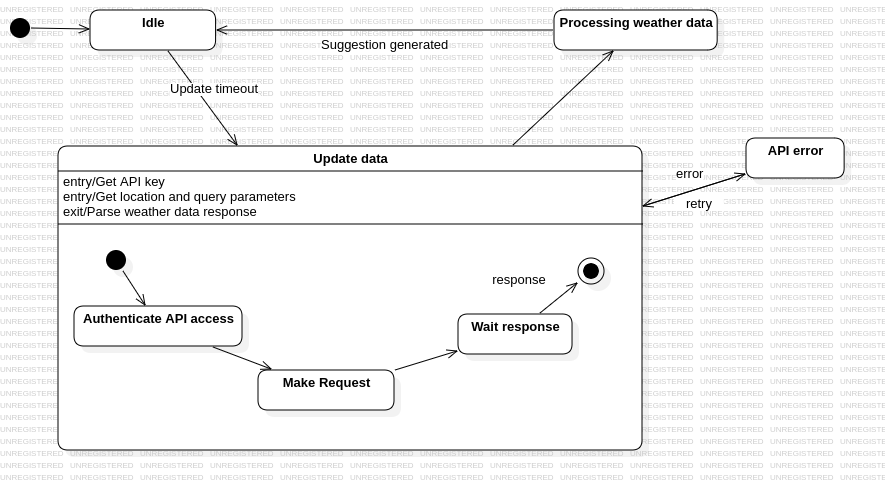
\includegraphics[width=1\textwidth]{UML Diagrams/StateDiagram_createsuggestions.png}
    \caption{State Diagram for "Get suggestion based on weather" use case}
    \label{fig:suggested_er}
\end{figure}

\section{Logical Database Requirements}

\begin{figure}[H]
    \centering
    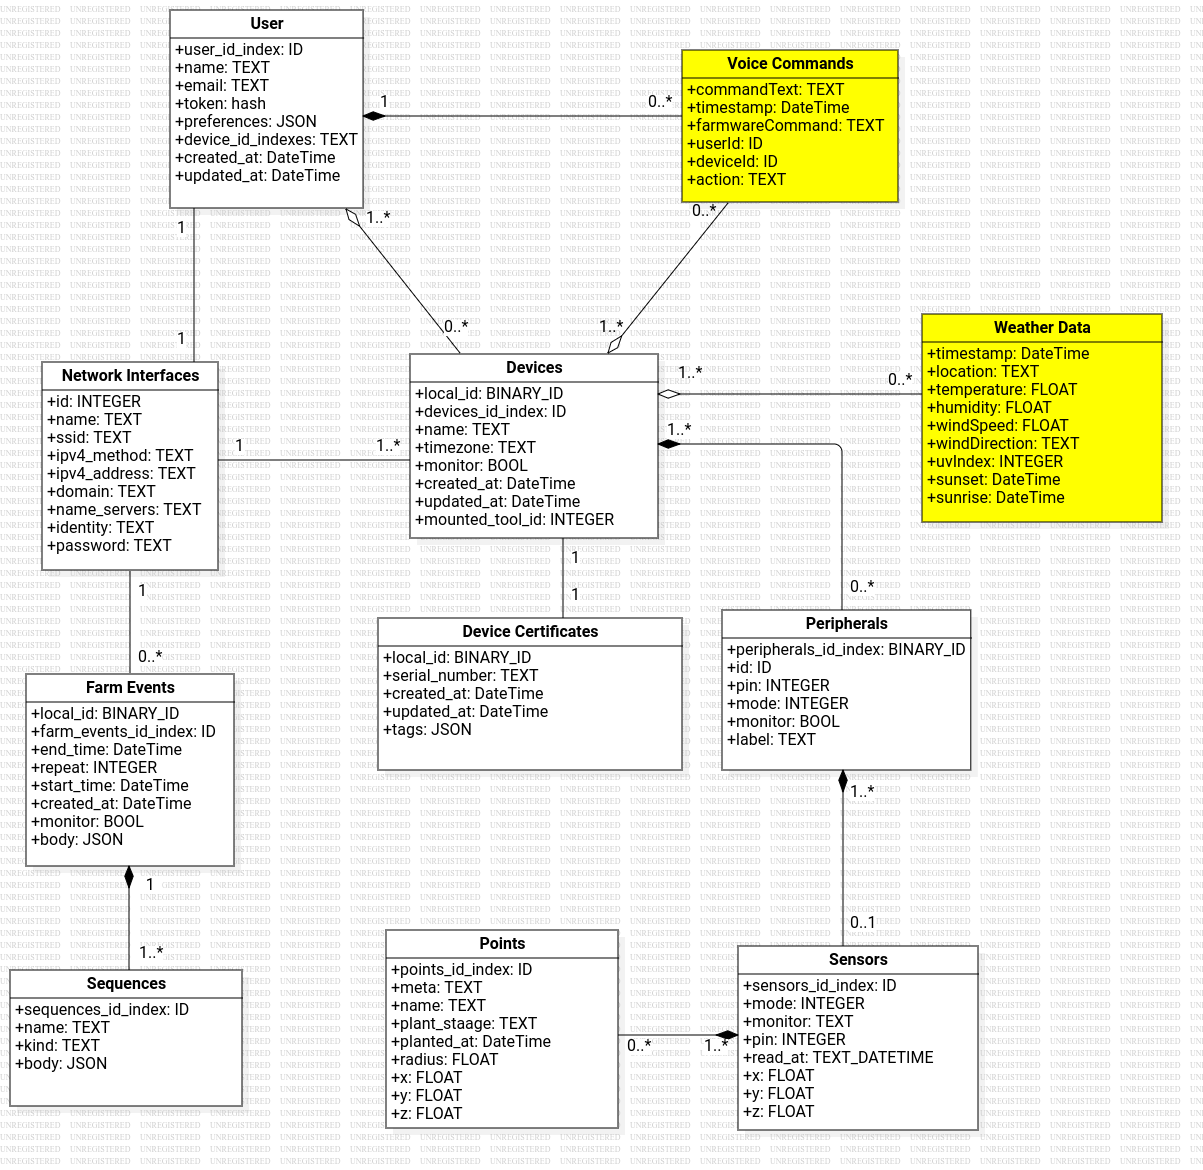
\includegraphics[width=1\textwidth]{UML Diagrams/SuggestedDBDiagram.png}
    \caption{Improved Logical Database Requirements Diagram}
    \label{fig:suggested_er}
\end{figure}

The improved logical database requirements diagram is shown in Figure \ref{fig:suggested_er}.
The system now has a new table named \textbf{Weather Data} to store weather data. This table has columns for weather data such as temperature, humidity, and wind speed. The system can store the weather data obtained from the Local Weather API in this table. Any device that has access to the database can read this data and use it to make better decisions for the farm.
\\
The system also has a new table named \textbf{Voice Commands} to store voice commands processed by the Voiceflow API. This table has columns for voice command data such as command text and action. The system can store the voice commands created by the user in this table. The system can read this data and execute the corresponding action when the user gives the voice command. A user may form their own voice commands and add them to the Voice Commands table and devices of this user can take action using the data stored in the Voice Commands table.

\section{Design Constraints}
\begin{itemize}
    \item FarmBot must ensure that the voice data taken from end user must be processed and used in a compliant manner with the data privacy regulations GDPR (General Data Protection Regulation), CCPA (California Consumer Privacy Act).
    \item FarmBot must ensure that data privacy regulations GDPR and CCPA are not breached during the acquisition of weather data from the Local Weather API by using users location information.
    \item Access to reliable, real-time weather data requires subscription to a trusted weather service, API.
    \item Development resources and expertise in speech recognition technology might be limited for the FarmBot project.
    \item Secure communication protocol SSL/TLS must be used to ensure user data protection and prevention of breaches while connecting to Alexa, Voiceflow and Weather API.
\end{itemize}

\section{System Quality Attributes}

\subsection{Usability Requirements}
\begin{itemize}
    \item Users should be able to successfully execute desired FarmBot actions using clear and concise voice commands.
    \item The voice recognition system should understand commands quickly and minimize the need for repeated attempts or corrections.
    \item The voice control interface should be intuitive and enjoyable to use, reducing reliance on manual controls.
    \item Farming action suggestions should be clear, actionable, and relevant to the user's specific farm context
    \item Weather data and suggestions should be presented concisely and easily understandable within the FarmBot interface.
    \item Users should find the suggestions helpful for making informed decisions about their farming actions.
    \item Voice control should support a variety of user accents and speaking styles.
\end{itemize}

\subsection{Performance Requirements}
\begin{itemize}
    \item Average time to execute the sequence indicated by the voice command shall not exceed 5 seconds to ensure user satisfaction.
    \item User shall not need to have to repeat their voice command more than 2 times.
    \item Voice command interpretation accuracy must be at least 95%.
    \item Weather forecasts for the coming day must be acquired daily at 2AM-4AM (FarmBot update hours) with a delay of no more than 10 minutes.
\end{itemize}

\subsection{Reliability}
\begin{itemize}
    \item Speech recognition must be accurate.
    \item Potential misinterpretations of voice commands must be handled gracefully, prompting for confirmation or offering alternative options must be implemented.
    \item Weather data source must have a high uptime and provide accurate weather information.
\end{itemize}

\subsection{Availability}
\begin{itemize}
    \item Voice control functionality must be highly available, downtime due to recognition engine issues must be minimized.
    \item Despite weather data feed not being available, system should remain functional and give suggestions based on historical data or user preferences.
\end{itemize}

\subsection{Security}
\begin{itemize}
    \item User voice data of any kind must be anonymized and opt-out option to users must be presented.
    \item Secure communication protocols such as HTTPS, SSL/TLS must be followed.
    \item FarmBot must not endanger its users due to misinterpreted voice commands
\end{itemize}

\subsection{Maintainability}
\begin{itemize}
    \item Voice control and weather modules must be designed as seperate, well-documented modules to facilitate future improvements or integrations with different speech recognition engines.
\end{itemize}

\subsection{Portability}
\begin{itemize}
    \item Speech recognition libraries, APIs used must be protable accros different platforms to maintain compatibility with potential hardware upgrades.
    \item Established libraries must be utilized for accessing and parsing weather data formats to ensure compatibility with various weather service APIs.
\end{itemize}

\section{Supporting Information}
In order to implement these suggestions the following choices are made: \\
Amazon Alexa is chosen as the hardware for capturing user voice and sending it to VoiceFlow for processing it. It supports various languages: English, German, Indian, Japanese, French, Italian, and Spanish ensuring accessibility for different cultures. \\
World Weather API's, "Local Weather API" is selected for the weather data source. It includes various metrics about the current weather at user's location such as temperature, humidity, and wind speed. The data is updated daily and it costs \$120 monthly for a million requests per day to the API. JSON format is used for acquiring and parsing the weather data.